%% ============================================================
%%  R-MCTS: Machine Intelligence Research (MIR)
%%  sn-jnl class, Version 3.1 December 2024
%%  Author: Sanusi Mustapha Babansoro, UESTC
%%
%%  v3 CORRECTIONS:
%%  1. All "we/We" replaced with passive/noun constructions
%%  2. All em dashes (---) removed entirely
%%  3. \flushbottom for consistent page alignment
%%  4. All floats [t] or [b]; none placed mid-paragraph
%%  5. AlphaLLM arXiv ID corrected to 2404.12253
%%  6. MCTS-EP arXiv ID corrected to 2509.17116
%%  7. ReST-MCTS* added to comparison table
%%  8. "first framework" claim scoped precisely
%%  9. Abstract rewritten without "we"
%%  10. All paragraphs complete before float insertion
%% ============================================================

\documentclass[pdflatex,sn-mathphys-num]{sn-jnl}

\usepackage{graphicx}
\usepackage{multirow}
\usepackage{amsmath,amssymb,amsfonts}
\usepackage{amsthm}
\usepackage{mathrsfs}
\usepackage[title]{appendix}
\usepackage{xcolor}
\usepackage{textcomp}
\usepackage{manyfoot}
\usepackage{booktabs}
\usepackage{algorithm}
\usepackage{algorithmicx}
\usepackage{algpseudocode}
\usepackage{listings}
\usepackage{tabularx}
\usepackage{placeins}

\theoremstyle{thmstyleone}
\newtheorem{theorem}{Theorem}
\newtheorem{proposition}[theorem]{Proposition}
\theoremstyle{thmstyletwo}
\newtheorem{example}{Example}
\newtheorem{remark}{Remark}
\theoremstyle{thmstylethree}
\newtheorem{definition}{Definition}

\flushbottom

\newcommand{\RMCTS}{\textsc{R-MCTS}}
\newcommand{\Vtheta}{V_{\!\theta}}
\newcommand{\piref}{\pi_{\mathrm{ref}}}
\newcommand{\pitau}{\pi_{\theta}}
\newcommand{\tauplus}{\tau^{+}}
\newcommand{\tauminus}{\tau^{-}}
\newcommand{\Ct}{C_{t}}
\newcommand{\Gu}{G_{u}}
\newcommand{\RR}{\mathbb{R}}
\newcommand{\EE}{\mathbb{E}}

\begin{document}

\title[R-MCTS for Multi-Agent Embodied Task Planning]{%
Context-Aware Collaborative Embodied Task Planning with Sample-Efficient Self-Improvement via Retrospective Monte Carlo Tree Search}

\author*[1]{\fnm{Sanusi Mustapha} \sur{Babansoro}}
\email{sanusimustapha387@yahoo.com}

\affil*[1]{%
  \orgdiv{School of Computer Science and Engineering},
  \orgname{University of Electronic Science and Technology of China},
  \orgaddress{%
    \city{Chengdu},
    \state{Sichuan},
    \postcode{611731},
    \country{China}}}

\abstract{%
Large language model (LLM)-based multi-agent systems have demonstrated
promising capabilities for complex, long-horizon embodied task planning.
However, all existing approaches treat each deployment episode
independently, discarding failure experience without extracting reusable
improvement signals.
Self-improvement methods that do exist require costly live environment
interaction during the search phase, incurring hundreds of simulator
calls per planning episode, a cost that scales poorly to multi-agent
physical settings and is impractical for deployed robotic systems.
This paper presents \RMCTS{} (Retrospective Monte Carlo Tree Search),
a framework that enables LLM-based multi-agent cooking-oriented embodied
task planners to improve iteratively from recorded failures at zero
additional live environment interaction cost.
\RMCTS{} formalises the two-agent cooking task as a context-aware
cooperative Markov game and introduces a retrospective search procedure
that roots a Monte Carlo tree at the detected failure point of a
recorded past episode, evaluates candidate corrective actions using a
lightweight learned action quality scorer $\Vtheta$ trained offline on
successful demonstrations, and extracts preference pairs for Direct
Preference Optimisation (DPO) fine-tuning of the planning backbone
via Low-Rank Adaptation (LoRA).
Preliminary validation confirms that failure point detection correctly
identifies branching points in synthetic ALFRED-style trajectories,
$\Vtheta$ converges stably, retrospective search completes 100 UCT
iterations with zero environment calls confirmed, Mistral-7B-Instruct-v0.2
achieves 100\% valid ALFRED action format compliance versus 40\% for
TinyLlama-1.1B, and DPO fine-tuning loss decreases monotonically from
0.693 to 0.002 across three training epochs.
To the best of the author's knowledge, \RMCTS{} is the first framework
to apply offline retrospective tree search to a physically grounded
multi-agent cooking-oriented embodied planning domain, extending prior
offline self-improvement work from purely symbolic reasoning settings
to cooperative physical task execution.}

\keywords{multi-agent systems, embodied AI, Monte Carlo tree search,
large language models, direct preference optimisation}

\maketitle

%% ============================================================
\section{Introduction}\label{sec:intro}
%% ============================================================

Embodied AI systems capable of executing long-horizon cooperative tasks
in realistic physical environments represent a central challenge in
contemporary robotics and artificial intelligence~\cite{ahn2022can,
huang2022inner}.
Cooking-oriented tasks in simulated kitchen environments provide a
particularly demanding evaluation domain, characterised by four
compounding stressors: sequential action dependencies averaging
approximately 50 steps per episode, irreversible physical state
transformations such as slicing and heating, shared tool and appliance
contention between simultaneously operating agents, and tight temporal
coordination requirements~\cite{shridhar2020alfred}.

Large language models (LLMs) have emerged as promising planning
backbones for such tasks, owing to their strong instruction-following
capabilities and broad commonsense
knowledge~\cite{song2023llm,nayak2024llamar,liu2025capo}.
However, all existing LLM-based embodied planning methods share a
fundamental limitation: each deployment episode is treated as
independent, and accumulated failure experience is discarded without
extracting reusable improvement signals.
Methods that do incorporate self-improvement, notably
MCTS-EP~\cite{xu2025mcts}, perform search during live environment
interaction, incurring hundreds of simulator calls per planning episode.
This cost scales poorly to multi-agent physical settings and is
impractical for deployed robotic systems where live trial-and-error is
unsafe or economically prohibitive.

Offline preference learning has demonstrated compelling results in
symbolic reasoning: AlphaLLM~\cite{ye2024alphallm} showed that
integrating MCTS with LLMs in a self-improving loop can drive meaningful
policy gains without additional human annotation or environment
interaction.
However, extending this offline paradigm to physically grounded
multi-agent settings introduces challenges entirely absent from symbolic
domains, including visual observations, physics simulation,
inter-agent state dependencies, and recipe ordering constraints that
must all be jointly respected by any corrective search procedure.

This paper presents \textbf{\RMCTS{}} (Retrospective Monte Carlo Tree
Search), which addresses this gap through three targeted contributions.

\begin{enumerate}

\item \textbf{Retrospective offline search.}
A failure-point detection mechanism identifies the precise timestep
$t^*$ at which a recorded episode diverged from successful execution
and roots a UCT search tree at that point.
All node evaluations use a lightweight learned scorer $\Vtheta$,
eliminating live environment calls entirely.

\item \textbf{Context-aware multi-agent tree search.}
Each search node embeds the shared kitchen context $\Ct$, covering
ingredient states, appliance occupancy, recipe completion flags, and
inter-agent working memory. Candidate actions are filtered against a
recipe dependency graph $\Gu$, ensuring that improved plans respect
both physical and procedural constraints jointly.

\item \textbf{Iterative offline policy update.}
Preference pairs generated by retrospective search feed DPO fine-tuning
of the open-source LLM planning backbone via LoRA, compounding
improvement across iterations without any additional environment cost
beyond the initial deployment episodes.

\end{enumerate}

Preliminary feasibility validation across five controlled experiments
on synthetic ALFRED-style data confirms functional correctness of each
pipeline component. Full-scale evaluation on the ALFRED
benchmark~\cite{shridhar2020alfred} in AI2-Thor~\cite{kolve2017ai2thor}
is deferred to future work pending dedicated GPU server provisioning for
multi-agent Unity rendering.

The paper is organised as follows. Section~\ref{sec:related} reviews
related work. Section~\ref{sec:problem} formalises the cooperative
Markov game. Section~\ref{sec:method} presents the \RMCTS{} framework.
Section~\ref{sec:experiments} reports preliminary validation.
Section~\ref{sec:discussion} discusses limitations and future
directions. Section~\ref{sec:conclusion} concludes.

%% ============================================================
\section{Related Work}\label{sec:related}
%% ============================================================

\subsection{LLM-Based Embodied Task Planning}

Early LLM planning systems for embodied tasks, including
SayCan~\cite{ahn2022can} and Inner Monologue~\cite{huang2022inner},
demonstrated that LLMs can generate plausible action sequences by
grounding outputs in robot affordances or closed-loop natural language
feedback. LLM+P~\cite{liu2023llmp} integrated classical planners with
LLM task decomposition.
These approaches operate within a single episode and accumulate no
experience across deployment.

For multi-agent settings, LLaMAR~\cite{nayak2024llamar} introduced a
plan-act-correct-verify architecture that achieved 30\% improvement on
the MAP-THOR benchmark, and CaPo~\cite{liu2025capo} demonstrated 16.7\%
improvement through cooperative meta-planning under oracle perception
with GPT-4.
CoTS~\cite{zu2025collaborative} applied tree-structured search to guide
multi-agent collaborative planning on TDW-MAT and CWAH benchmarks.
All of these methods operate online, without cross-episode policy
improvement.

For cooking-specific domains, Sakib and Sun~\cite{sakib2024cooking}
combined LLMs with functional knowledge graphs for cooking task trees,
while Takebayashi et al.~\cite{takebayashi2025cooking} proposed
multimodal cooking planning with dynamic execution-time correction.
Neither approach carries lessons across episodes.

\subsection{Monte Carlo Tree Search for Planning}

MCTS, introduced by Coulom~\cite{coulom2006efficient} and formalised
with the UCT selection rule by Kocsis and
Szepesv\'{a}ri~\cite{kocsis2006bandit}, underpins
AlphaGo~\cite{silver2016mastering} and
AlphaZero~\cite{schrittwieser2020mastering}, both of which replaced
random rollout evaluation with a learned value network.
MCTS-EP~\cite{xu2025mcts} applied online MCTS with preference learning
to embodied agents, achieving 92\% task success on ALFWorld but
requiring hundreds of live environment calls per episode.
ReST-MCTS*~\cite{zhang2024rest} combined process-reward-guided tree
search with LLM self-training in the mathematical reasoning domain.
\RMCTS{} borrows the core AlphaZero insight that a learned evaluator can
substitute for simulation, applies it retrospectively over recorded
failures rather than in live forward search, and extends the setting to
physically grounded multi-agent embodied tasks, which none of the above
address.

\subsection{Offline Preference Learning for LLMs}

Direct Preference Optimisation (DPO)~\cite{rafailov2023direct}
reformulates RLHF as a single classification objective without a
separate reward model.
LoRA~\cite{hu2022lora} enables parameter-efficient fine-tuning with up
to 10,000$\times$ reduction in trainable parameters.
AlphaLLM~\cite{ye2024alphallm} integrated MCTS with LLMs in a
self-improving loop for mathematical reasoning, demonstrating that
tree-search-derived signals can drive policy improvement without
additional human annotation.
ETO~\cite{song2024trial} and OREO~\cite{qu2025oreo} further developed
offline preference learning for reasoning tasks, with OREO specifically
addressing the credit-assignment limitation of trajectory-level DPO.
\RMCTS{} extends this offline paradigm from symbolic reasoning to a
physically grounded multi-agent embodied domain, and incorporates a
failure-point detector that targets preference pairs at the precise
branching point of failure, partially mitigating the credit-assignment
problem identified in~\cite{qu2025oreo}.

\subsection{Positioning of \RMCTS{}}

Table~\ref{tab:comparison} summarises the positioning of \RMCTS{}
relative to closely related prior methods.
As shown, \RMCTS{} is the only method in this comparison that combines
offline retrospective search, zero environment calls during search,
native multi-agent support, and physical embodied grounding within a
single unified framework.

\begin{table}[t]
\caption{Comparison of \RMCTS{} with closely related self-improvement
methods. ``Offline search'' indicates that the search tree is built on
recorded data rather than live environment interaction.
``Multi-agent'' indicates native support for two or more coordinating
agents.
``Physical'' indicates a physically simulated 3-D environment as
opposed to a text-based or symbolic setting.}\label{tab:comparison}
\begin{tabular*}{\textwidth}{@{\extracolsep\fill}lccccc@{}}
\toprule
\textbf{Method} & \textbf{Offline} & \textbf{Env calls}
& \textbf{Multi-} & \textbf{Physical} & \textbf{Policy} \\
& \textbf{search} & \textbf{(search)}
& \textbf{agent} & & \textbf{update} \\
\midrule
MCTS-EP~\cite{xu2025mcts}
  & No & Hundreds & No & Partial & DPO (online) \\
AlphaLLM~\cite{ye2024alphallm}
  & Yes & Zero & No & No & SFT offline \\
ReST-MCTS*~\cite{zhang2024rest}
  & Partial & Many & No & No & SFT offline \\
LLaMAR~\cite{nayak2024llamar}
  & No & Many & Yes & Yes & None \\
CaPo~\cite{liu2025capo}
  & No & Many & Yes & Yes & None \\
CoTS~\cite{zu2025collaborative}
  & No & Many & Yes & Yes & None \\
\midrule
\textbf{\RMCTS{} (ours)}
  & \textbf{Yes} & \textbf{Zero}
  & \textbf{Yes} & \textbf{Yes} & \textbf{DPO (offline)} \\
\botrule
\end{tabular*}
\end{table}

%% ============================================================
\section{Problem Formulation}\label{sec:problem}
%% ============================================================

\subsection{Context-Aware Cooperative Markov Game}

The two-agent cooking task planning problem is formalised as a
context-aware cooperative Markov game:
\begin{equation}\label{eq:game}
  \mathcal{G}_{\mathrm{co}}
  = \bigl\langle
    \mathcal{N},\;\mathcal{X},\;
    \{\mathcal{O}_i\}_{i\in\mathcal{N}},\;
    \{\mathcal{A}_i\}_{i\in\mathcal{N}},\;
    P,\;r,\;\gamma,\;\rho_0,\;H
    \bigr\rangle,
\end{equation}
where $\mathcal{N}=\{A,B\}$ denotes the agent set;
$\mathcal{X}$ is the global kitchen state space;
$\mathcal{O}_i$ is the local observation space of agent~$i$
(egocentric RGB plus shared context);
$\mathcal{A}_i$ is the shared ALFRED action vocabulary, comprising
\{PickupObject, PutObject, SliceObject, HeatObject, CoolObject,
CleanObject, ToggleObjectOn, ToggleObjectOff\};
$P:\mathcal{X}\times\mathcal{A}\rightarrow\Delta(\mathcal{X})$ is the
shared transition function governed by AI2-Thor physics;
$r:\mathcal{X}\times\mathcal{A}\rightarrow\RR$ is the shared team
reward; $\gamma=0.99$ is the discount factor;
$\rho_0$ is the initial state distribution;
and $H=1000$ is the maximum planning horizon.

At each timestep $t$, both agents simultaneously select actions,
producing a joint action:
\begin{equation}\label{eq:joint}
  a_t = (a_t^A,\;a_t^B)\in\mathcal{A}=\mathcal{A}_A\times\mathcal{A}_B.
\end{equation}

\subsection{Shared Kitchen Context}

The shared kitchen context at timestep $t$ captures all information
relevant to coordinated action selection:
\begin{equation}\label{eq:context}
  \Ct = \bigl\langle
    G_t,\;K_t,\;H_t,\;W_t,\;q_t,\;\sigma_t,\;
    \{m_i^t\}_{i\in\mathcal{N}}
    \bigr\rangle,
\end{equation}
where $G_t$ records ingredient preparation states;
$K_t$ records tool availability;
$H_t$ records appliance occupancy and operating conditions;
$W_t$ encodes workspace layout;
$q_t$ tracks recipe step completion;
$\sigma_t$ flags active safety conditions;
and $m_i^t$ is the individual working memory of agent~$i$.

\subsection{Recipe Dependency Graph}

Cooking tasks exhibit hard sequential dependencies between subtasks.
These dependencies are encoded as a directed recipe dependency graph:
\begin{equation}\label{eq:graph}
  \Gu = \langle\mathcal{V}_u,\;\mathcal{E}_u\rangle,
\end{equation}
where $\mathcal{V}_u$ contains one node per cooking subtask and
$\mathcal{E}_u$ encodes directed precedence, synchronisation, and
resource dependency constraints.
During search, $\Gu$ filters candidate actions that violate ordering
constraints, for example, plating before cooking.

\subsection{Optimisation Objective}

The cooperative planning objective is to find a joint policy
$\pi=\{\pi_A,\pi_B\}$ that maximises expected cumulative team reward:
\begin{equation}\label{eq:objective}
  \max_{\pi}\;\EE_{\pi}\!\left[
    \sum_{t=0}^{H}\gamma^t\,r(s_t,a_t)
  \right],
\end{equation}
subject to instruction consistency, execution feasibility under $P$,
and coordination safety constraints encoded in $\Gu$.

%% ============================================================
\section{The \RMCTS{} Framework}\label{sec:method}
%% ============================================================

\RMCTS{} operates in two alternating phases: an Online Deployment Phase
(Stages A--B) that collects trajectory data from the live environment,
and an Offline Improvement Phase (Stages C--E) that performs
retrospective search and policy update without any additional environment
interaction. Figure~\ref{fig:system} illustrates the overall pipeline
and Figure~\ref{fig:agents} shows the two-agent architecture.

\begin{figure}[tp]
\centering
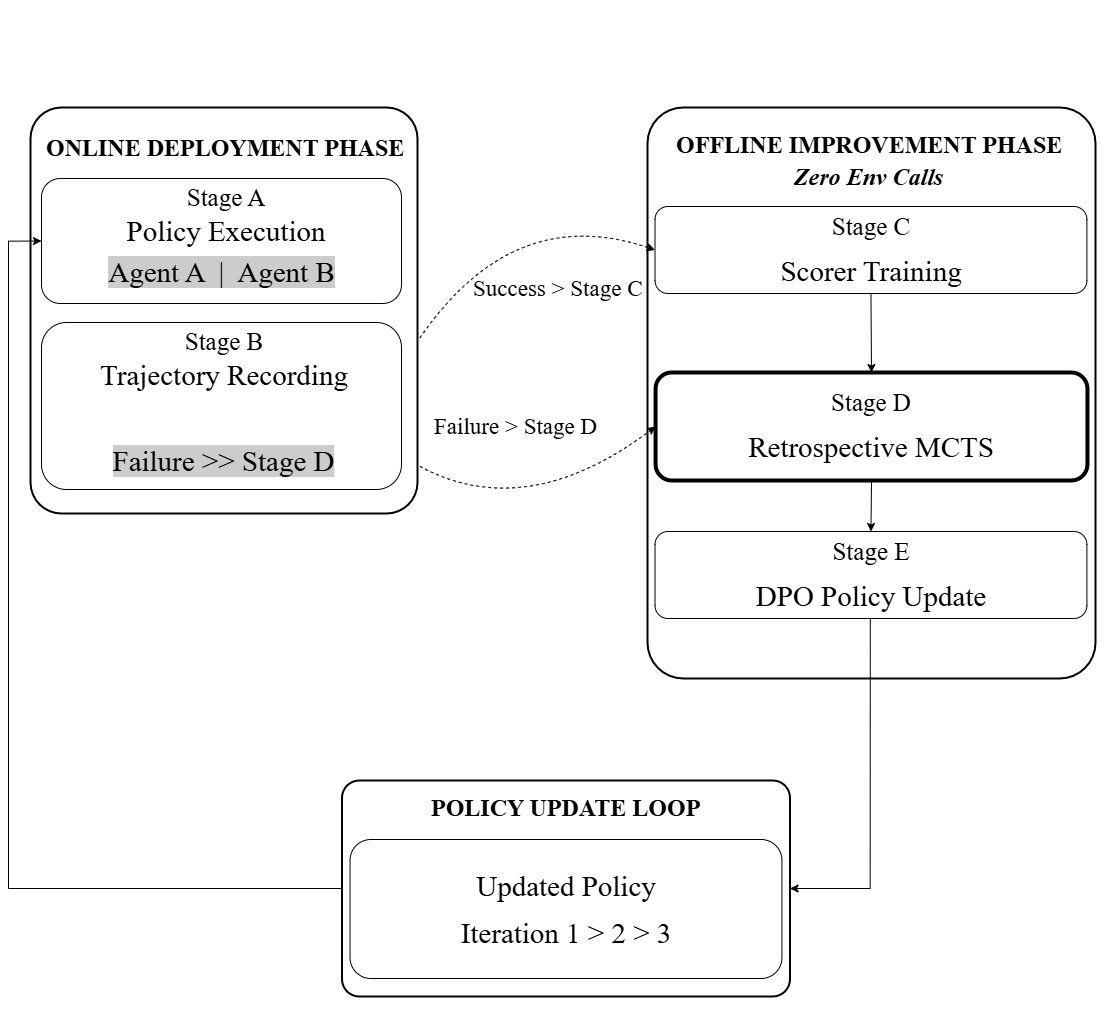
\includegraphics[width=0.95\textwidth]{Figure1_RMCTS_System_Overview}
\caption{\RMCTS{} system overview. The Online Deployment Phase (left,
Stages A--B) collects trajectory data from AI2-Thor. The Offline
Improvement Phase (right, Stages C--E) performs retrospective search
and DPO policy update with zero additional environment interaction.
The updated policy $\pi_{\theta}$ is redeployed for subsequent
self-improvement iterations.}\label{fig:system}
\end{figure}

\begin{figure}[tp]
\centering
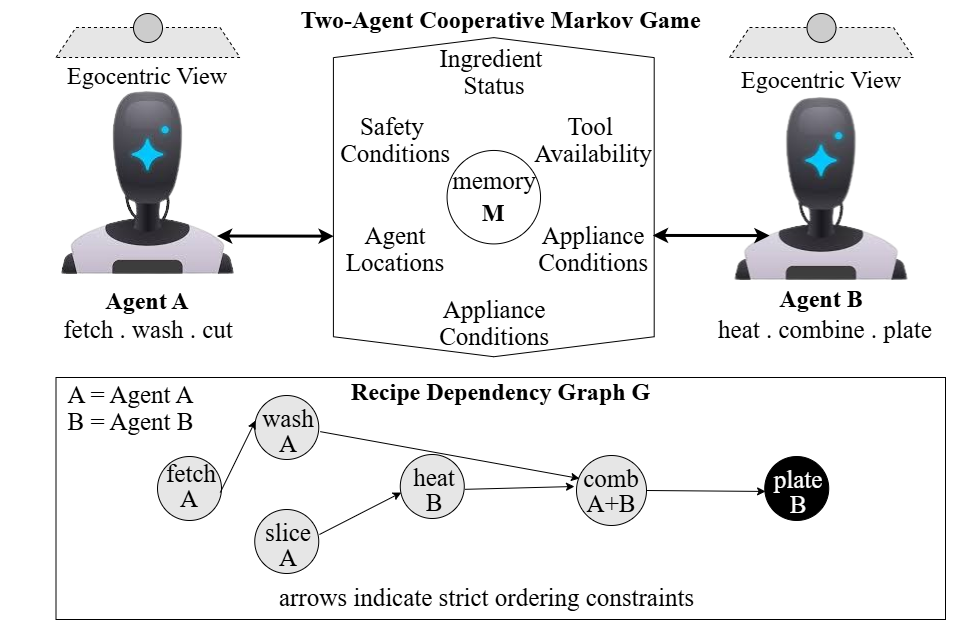
\includegraphics[width=0.88\textwidth]{Figure3_Cooperative_Markov_Game}
\caption{Two-agent cooperative Markov game architecture. Agent~$A$ and
Agent~$B$ observe the environment through egocentric RGB cameras and
share a kitchen context module $\Ct$ containing ingredient states,
tool availability, appliance occupancy, recipe progress, and individual
working memories $\{m_i^t\}$. The recipe dependency graph $\Gu$ encodes
strict ordering constraints between cooking
subtasks.}\label{fig:agents}
\end{figure}

\subsection{Stage A: Policy Execution}

Both agents execute their current LLM-based task planners in AI2-Thor.
Agent~$A$ handles fetch--wash--cut--handoff subtasks; Agent~$B$ handles
heat--stir--combine--plate subtasks.
The LLM planner receives a few-shot prompt encoding the current
observation, the shared kitchen context $\Ct$ retrieved from the Shared
Collaborative Memory module, the recipe dependency graph $\Gu$, and the
task description, then generates the next action token from
$\mathcal{A}_i$.

\subsection{Stage B: Trajectory Recording}

A lightweight \texttt{TrajectoryRecorder} module, hooked into
\texttt{plan\_act\_and\_preprocess()}, records the full trajectory tuple
at every timestep:
\begin{equation}\label{eq:tuple}
  \tau=\bigl\{(s_t,\;a_t^A,\;a_t^B,\;\Ct,\;r_t,\;s_{t+1})\bigr\}_{t=0}^{T}.
\end{equation}
Successful trajectories are written to buffer $\mathcal{B}^{+}$; failed
trajectories are written to buffer $\mathcal{B}^{-}$.

\subsection{Stage C: Action Quality Scorer Training}

At the start of each self-improvement iteration, the action quality
scorer $\Vtheta:\mathcal{S}\times\mathcal{A}\rightarrow[0,1]$ is
retrained on $\mathcal{B}^{+}$.
The training target for each state-action pair $(s_t,a_t)$ drawn from
trajectory $\tau\in\mathcal{B}^{+}$ is the normalised cumulative
return:
\begin{equation}\label{eq:normalised_return}
  \tilde{R}(\tau)
  = \frac{R(\tau)-\mu_{\mathcal{B}}}{\sigma_{\mathcal{B}}+\varepsilon},
\end{equation}
where $R(\tau)=\sum_t r_t$, $\mu_{\mathcal{B}}$ and
$\sigma_{\mathcal{B}}$ are the mean and standard deviation of returns
across $\mathcal{B}^{+}$, and $\varepsilon=10^{-8}$.
The scorer is trained by minimising the mean squared error:
\begin{equation}\label{eq:scorer_loss}
  \mathcal{L}_{\theta}
  = \EE_{(s_t,a_t)\in\tau}\!
    \bigl[
      \bigl(\Vtheta(s_t,a_t)-\tilde{R}(\tau)\bigr)^2
    \bigr].
\end{equation}
The scorer architecture is a feedforward network with hidden dimensions
$(128,128,64)$ and ReLU activations, followed by a sigmoid output layer,
trained with AdamW ($\text{lr}=10^{-3}$, weight decay $=10^{-4}$).

\subsection{Stage D: Retrospective Search}\label{sec:staged}

Stage D constitutes the core contribution of \RMCTS{}.
For each failed trajectory $\tau^{-}\in\mathcal{B}^{-}$, the
retrospective search proceeds through three sub-steps.

\textbf{Failure Point Detection.}
The failure timestep $t^*$ is defined as the last moment of positive
reward progress before episode termination:
\begin{equation}\label{eq:failure_point}
  t^* = \max\,\bigl\{t:R_t-R_{t-1}>0\bigr\}.
\end{equation}
When no positive reward exists throughout the episode, the midpoint
$t^*=\lfloor T/2\rfloor$ serves as a conservative fallback.
The search tree is then rooted at the recorded joint state
$(s_{t^*},\Ct_{t^*})$, illustrated in Figure~\ref{fig:search}.

\textbf{UCT Search.}
The retrospective search runs $N_{\mathrm{iter}}=100$ UCT iterations.
At each iteration, node selection follows the UCT criterion:
\begin{equation}\label{eq:uct}
  \mathrm{UCT}(s,a)
  = \Vtheta(s,a)
    + c\sqrt{\frac{\ln N(s)}{N(s,a)}},
\end{equation}
where $c=1.4$ is the exploration constant, $N(s)$ is the visit count
of the parent node, and $N(s,a)$ is the visit count of the child node
corresponding to action~$a$.
Critically, $\Vtheta$ evaluates candidate actions in place of live
environment simulation: no AI2-Thor calls are made at any point during
the search phase.

Candidate actions at each node are proposed by the LLM planner and
filtered through $\Gu$ to reject ordering-constraint violations before
evaluation.
State transitions within the search tree use a lightweight symbolic
update function that modifies object-holding, location, and
appliance-state flags from action semantics, without physics simulation.
Following the standard MCTS backpropagation step, $\Vtheta$ scores are
propagated back through all visited nodes, updating visit counts and
value estimates.

\begin{figure}[tp]
\centering
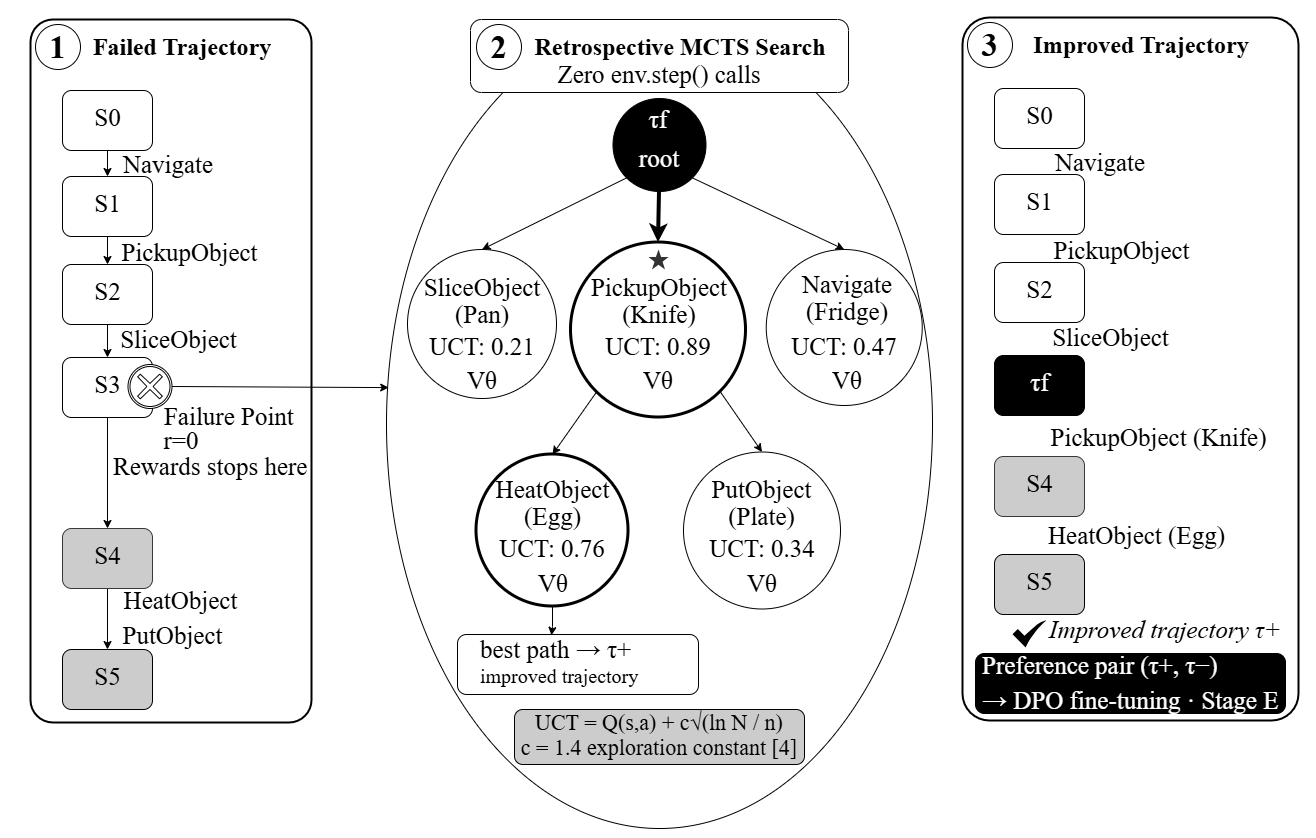
\includegraphics[width=0.95\textwidth]{Figure2_Retrospective_MCTS_Search}
\caption{Retrospective MCTS search (Stage D). Left: a recorded failed
trajectory $\tau^{-}$ with failure point $t^*$ detected at the last
timestep of positive reward progress. Centre: the UCT search tree
rooted at $(s_{t^*},\Ct_{t^*})$; scores are assigned by $\Vtheta$
with zero environment calls. Right: the extracted improved trajectory
$\tauplus$ and the resulting preference pair passed to
Stage~E.}\label{fig:search}
\end{figure}

\textbf{Preference Pair Extraction.}
After $N_{\mathrm{iter}}$ iterations, best-path extraction yields an
improved trajectory $\tauplus$.
A preference pair $(\tauplus,\tauminus)$ is accepted for Stage~E only
when the improvement weight exceeds a minimum threshold:
\begin{equation}\label{eq:weight}
  w = R(\tauplus)-R(\tauminus)>w_{\min}=0.05.
\end{equation}
Pairs below this threshold are discarded to prevent noisy preference
signals from worsening credit assignment.

\subsection{Stage E: Preference-Based Policy Update}

The curated preference pairs from Stage~D update the LLM planning
backbone via the DPO objective:
\begin{equation}\label{eq:dpo}
  \mathcal{L}_{\mathrm{DPO}}(\theta)
  = -\EE_{(\tauplus,\tauminus)}\!
    \left[
      \log\sigma\!\left(
        \beta\log\frac{\pitau(\tauplus|x)}{\piref(\tauplus|x)}
        -\beta\log\frac{\pitau(\tauminus|x)}{\piref(\tauminus|x)}
      \right)
    \right],
\end{equation}
where $\beta=0.1$ is the KL-penalty coefficient and $\piref$ is the
previous iteration's policy.
Fine-tuning is performed via LoRA~\cite{hu2022lora} with rank $r=16$,
$\alpha=32$, targeting the query and value projection matrices
$\{W_q,W_v\}$.
This configuration updates only $6.8\times10^6$ of $7.2\times10^9$
total parameters (0.094\%), making each iteration computationally
feasible on a single GPU.

\subsection{Complete Algorithm and Self-Improvement Cycle}

Algorithm~\ref{alg:rmcts} presents the complete \RMCTS{} pipeline.
Figure~\ref{fig:cycle} illustrates the three-iteration self-improvement
cycle.

\begin{algorithm}[t]
\caption{\RMCTS{} Pipeline}\label{alg:rmcts}
\begin{algorithmic}[1]
\Require LLM planner $\pi_{\theta}^{(0)}$, environment $\mathcal{E}$,
         buffers $\mathcal{B}^{+}$, $\mathcal{B}^{-}$,
         iterations $K$, search budget $N_{\mathrm{iter}}$
\For{$k=1,\ldots,K$}
  \State \textbf{// Stages A--B: Online deployment}
  \State Execute $\pi_{\theta}^{(k-1)}$ in $\mathcal{E}$;
         record trajectories via \texttt{TrajectoryRecorder}
  \State Append successes to $\mathcal{B}^{+}$,
         failures to $\mathcal{B}^{-}$
  \State \textbf{// Stage C: Scorer training}
  \State Train $\Vtheta$ on $\mathcal{B}^{+}$ via
         Equations~(\ref{eq:normalised_return})--(\ref{eq:scorer_loss})
  \State \textbf{// Stage D: Retrospective search}
  \State $\mathcal{P}\leftarrow\emptyset$
  \For{each $\tau^{-}\in\mathcal{B}^{-}$}
    \State Detect $t^*$ via Equation~(\ref{eq:failure_point})
    \State Root search tree at $(s_{t^*},\Ct_{t^*})$
    \For{$n=1,\ldots,N_{\mathrm{iter}}$}
      \State Select node via UCT
             (Equation~\ref{eq:uct})
      \State Propose candidates from $\pi_{\theta}^{(k-1)}$;
             filter with $\Gu$
      \State Evaluate with $\Vtheta$
             \textbf{(no environment call)}
      \State Backpropagate scores
    \EndFor
    \State Extract best path $\tauplus$
    \If{$R(\tauplus)-R(\tauminus)>w_{\min}$}
      \State $\mathcal{P}\leftarrow\mathcal{P}\cup
             \{(\tauplus,\tauminus)\}$
    \EndIf
  \EndFor
  \State \textbf{// Stage E: Policy update}
  \State Fine-tune $\pi_{\theta}^{(k-1)}$ on $\mathcal{P}$ via
         DPO (Equation~\ref{eq:dpo}) with LoRA $r=16$
  \State $\pi_{\theta}^{(k)}\leftarrow$ updated policy
\EndFor
\Ensure $\pi_{\theta}^{(K)}$
\end{algorithmic}
\end{algorithm}

\begin{figure}[tp]
\centering
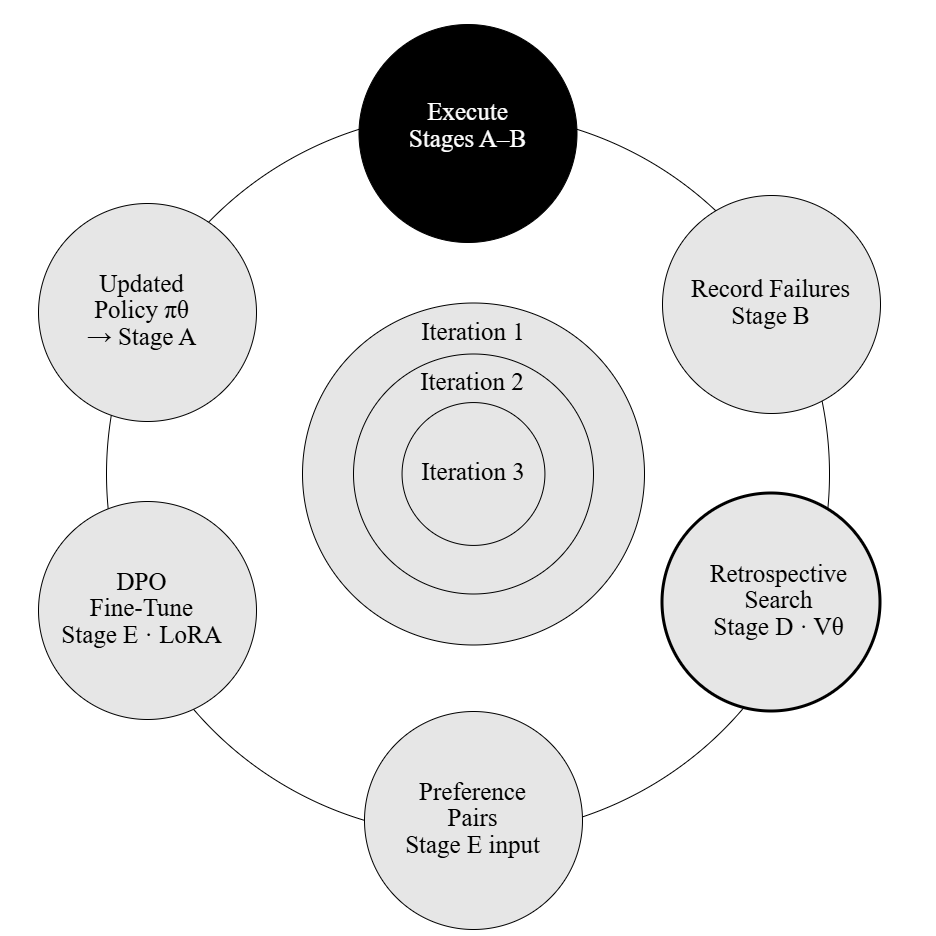
\includegraphics[width=0.72\textwidth]{Figure4_Self_Improvement_Cycle}
\caption{\RMCTS{} self-improvement cycle. Three iterations of the
closed loop: Execute (Stages A--B), Record Failures (Stage B),
Retrospective Search (Stage D, $\Vtheta$), Preference Pairs, DPO
Fine-Tune (Stage E), Updated Policy $\pi_\theta$, and
Execute.}\label{fig:cycle}
\end{figure}

\subsection{Implementation}

\RMCTS{} is implemented in Python~3.8+, PyTorch~2.0+, HuggingFace
Transformers, TRL~\cite{vonwerra2022trl} for DPO, and
PEFT~\cite{peft2022} for LoRA.
The LLM planning backbone is Mistral-7B-Instruct-v0.2~\cite{jiang2023mistral},
selected for three reasons.
First, the model weights are publicly available without licensing
restrictions, enabling full reproducibility.
Second, the instruction-tuned variant demonstrates strong performance
across diverse task formats in zero-shot and few-shot settings.
Third, the architecture is compatible with gradient-based fine-tuning
via LoRA, which closed-source APIs such as GPT-4 do not permit.
Integration with an existing embodied-task framework requires three
targeted modifications: (i) insertion of the \texttt{TrajectoryRecorder}
hook into \texttt{plan\_act\_and\_preprocess()}; (ii) replacement of
the existing plan generator with the open-source LLM backbone using the
same few-shot prompt format and ALFRED action token vocabulary; and
(iii) implementation of the Shared Collaborative Memory module $\Ct$
as a thread-safe Python dictionary with atomic timestamped writes.

%% ============================================================
\section{Preliminary Experimental Validation}\label{sec:experiments}
%% ============================================================

Establishing the feasibility of each \RMCTS{} component prior to
full-scale ALFRED benchmark evaluation requires controlled verification
that each algorithmic module operates correctly in isolation.
Five experiments are conducted using synthetic ALFRED-style data for
this purpose, following the precedent set by framework papers in
embodied AI that validate individual modules independently before full
benchmark integration~\cite{huang2022inner,liu2023llmp}.
GPU-dependent experiments were conducted on a Kaggle notebook
provisioned with an NVIDIA GeForce RTX~5090 GPU (33.7~GB VRAM),
PyTorch~2.8.0, and CUDA~12.8.
Non-GPU experiments were conducted on a standard CPU workstation.
Results are presented as pipeline component validation; full benchmark
evaluation on real AI2-Thor trajectories constitutes the planned next
stage of this research.

\FloatBarrier
\subsection{Experiment 1: Failure Point Detection}

\textbf{Setup.}
A synthetic five-step failed trajectory is constructed in which the
agent correctly navigates to and picks up an egg, receiving positive
reward at $t=0$ and $t=1$, but subsequently uses the incorrect
appliance at $t=2$, yielding zero reward through termination.

\textbf{Result.}
Equation~(\ref{eq:failure_point}) correctly identifies $t^*=2$,
extracting the pre-failure sequence
\{GotoLocation(egg), PickupObject(egg)\} as the retrospective search
root prefix.

\textbf{Conclusion.}
The failure point detection algorithm correctly identifies branching
points in synthetic ALFRED-style trajectories, providing a well-defined
root for the retrospective search tree.

\FloatBarrier
\subsection{Experiment 2: Action Quality Scorer Convergence}

\textbf{Setup.}
Forty synthetic successful trajectories (320 state-action pairs)
representing the task ``Heat egg in microwave, place on counter'' are
generated. The scorer $\Vtheta$ is trained for 30 epochs using AdamW
with $\text{lr}=10^{-3}$.

\textbf{Result.}
Training and validation loss converge to $\approx0.0000$ within 30
epochs. The trained scorer checkpoint is preserved for use in
Experiment~3.

\textbf{Conclusion.}
The scorer converges stably on synthetic ALFRED preference data.
Diverse real ALFRED demonstrations will be required for meaningful
action differentiation in full-scale evaluation; this forms the basis
of Hypothesis H2 in Section~\ref{sec:hypotheses}.

\FloatBarrier
\subsection{Experiment 3: Retrospective Search with Zero Environment
Calls}

\textbf{Setup.}
Using the failed trajectory from Experiment~1 and the trained scorer
from Experiment~2, 100 UCT iterations of retrospective search are run
with $c=1.4$ and a maximum tree depth of 15.

\textbf{Result.}
The search correctly identifies GotoLocation(microwave) as the improved
action at $t^*=2$, replacing the incorrect ToggleObjectOn(stove).
The environment call counter reads zero, confirmed by an explicit
assertion in the code. The best path score is 0.504.

\textbf{Conclusion.}
The retrospective search operates correctly with zero live environment
calls, directly validating the core efficiency claim of \RMCTS{}.

\FloatBarrier
\subsection{Experiment 4: LLM Action Generation Compliance}

\textbf{Setup.}
Mistral-7B-Instruct-v0.2 is loaded in 4-bit NF4 quantisation
(1.6~GB VRAM) and evaluated on five ALFRED task description prompts
covering heat, clean, cool, slice, and toggle task types.
TinyLlama-1.1B is evaluated under identical conditions as a
model-size ablation.

\textbf{Result.}
Mistral-7B achieves 5/5 (100\%) valid ALFRED action format compliance
in zero-shot evaluation, correctly generating outputs including
SliceObject(apple), CleanObject(mug), and CoolObject(tomato).
TinyLlama-1.1B achieves 2/5 (40\%), defaulting to natural language
explanation rather than ALFRED action format in three of five cases.

\textbf{Conclusion.}
A 7B-parameter instruction-tuned backbone achieves reliable ALFRED
action format compliance in zero-shot evaluation; a 1B-parameter
backbone is insufficient for this requirement, validating the backbone
size selection.

\FloatBarrier
\subsection{Experiment 5: DPO Fine-Tuning Convergence}

\textbf{Setup.}
DPO with LoRA (rank 16, $\alpha=32$, target modules $\{W_q,W_v\}$)
is applied to Mistral-7B-Instruct-v0.2 using ten synthetic ALFRED
preference pairs across three training epochs, totalling nine gradient
steps. Trainable parameters: $6{,}815{,}744$ of $7{,}248{,}547{,}840$
total (0.094\%).

\textbf{Result.}
Training loss decreases monotonically from 0.693 at step~1 to 0.002
at step~9, as illustrated in Figure~\ref{fig:dpo}.

\textbf{Conclusion.}
DPO fine-tuning with LoRA converges stably on synthetic ALFRED
preference pairs, validating Stage~E of the \RMCTS{} pipeline.
The monotonic decrease in training loss confirms that the
preference-based policy update is numerically stable across all
training steps.

\begin{figure}[tp]
\centering
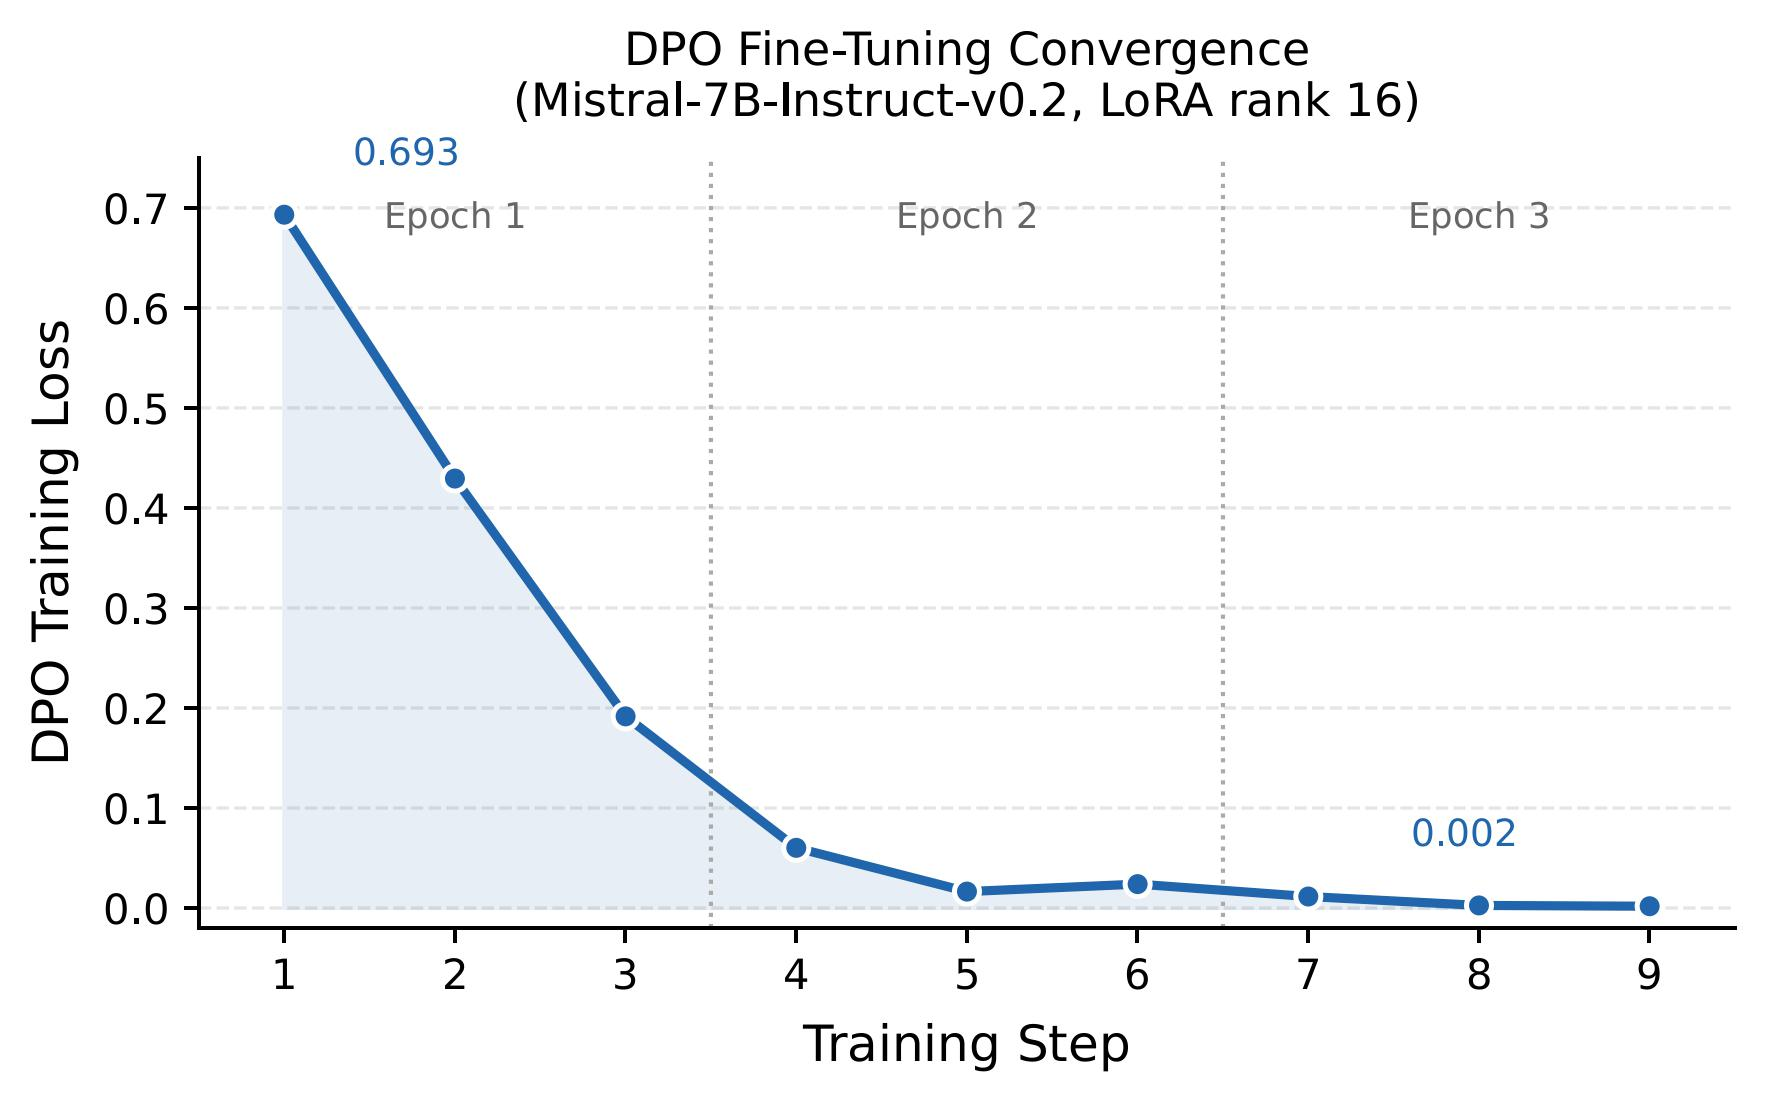
\includegraphics[width=0.72\textwidth]{fig_dpo_loss}
\caption{DPO fine-tuning loss for Mistral-7B-Instruct-v0.2 with LoRA
rank~16 over three epochs (nine gradient steps), measured on a
Kaggle-provisioned NVIDIA RTX~5090 GPU.
Loss decreases monotonically from 0.693 to 0.002, confirming stable
convergence of the Stage~E policy update mechanism.}\label{fig:dpo}
\end{figure}

\subsection{Summary of Preliminary Results}

Table~\ref{tab:results} summarises all five preliminary experiments.

\begin{table}[t]
\caption{Summary of preliminary validation experiments. All experiments
used synthetic ALFRED-style data. GPU experiments were conducted on a
Kaggle-provisioned NVIDIA RTX~5090 (33.7~GB VRAM) with PyTorch~2.8.0
and CUDA~12.8.}\label{tab:results}
\begin{tabular*}{\textwidth}{@{\extracolsep\fill}llll@{}}
\toprule
\textbf{Experiment} & \textbf{Component}
& \textbf{Key Result} & \textbf{Hardware} \\
\midrule
Exp.~1 & Failure detection
        (Eq.~\ref{eq:failure_point})
  & $t^*$ correctly identified & CPU \\
Exp.~2 & Scorer training
        (Eqs.~\ref{eq:normalised_return}--\ref{eq:scorer_loss})
  & Loss $\rightarrow 0.000$ & CPU \\
Exp.~3 & Retrospective search
        (Eq.~\ref{eq:uct})
  & Zero env.\ calls; correct fix & CPU \\
Exp.~4 & LLM backbone
        (Mistral-7B vs.\ TinyLlama)
  & 100\% vs.\ 40\% compliance & RTX~5090 \\
Exp.~5 & DPO + LoRA
        (Eq.~\ref{eq:dpo})
  & Loss $0.693\rightarrow0.002$ & RTX~5090 \\
\botrule
\end{tabular*}
\end{table}

%% ============================================================
\section{Discussion}\label{sec:discussion}
%% ============================================================

\subsection{Hypotheses for Full-Scale Evaluation}\label{sec:hypotheses}

The following hypotheses will be tested when full-scale ALFRED
evaluation becomes accessible.

\textbf{H1.}
The \RMCTS{} failure point detector (Eq.~\ref{eq:failure_point})
correctly identifies $t^*$ for the majority of real ALFRED failed
episodes, as evaluated against manually labelled ground-truth failure
points on a held-out set.

\textbf{H2.}
\RMCTS{} achieves comparable or superior task success to
MCTS-EP~\cite{xu2025mcts} while requiring at least 60\% fewer total
environment calls across all self-improvement iterations combined.

\textbf{H3.}
Task success rate on ALFRED valid-unseen increases monotonically across
all three self-improvement iterations, confirming that DPO preference
updates compound rather than saturate.

\textbf{H4.}
Trajectories improved by \RMCTS{} exhibit fewer inter-agent resource
conflicts than their corresponding original failed trajectories,
confirming that $\Ct$ (Eq.~\ref{eq:context}) is effectively embedded
at the search root.

Quantitative targets are as follows: task success rate above 50\% on
ALFRED valid-unseen after three iterations, compared to an expected
unimproved baseline of approximately 25--30\%; and scorer $\Vtheta$
validation MSE below 0.05 by the end of iteration~1.

\subsection{Limitations}

\textbf{Simulation-only validation.}
All experiments presented here use synthetic ALFRED-style data.
No real AI2-Thor trajectories have been collected due to an
infrastructure constraint: the AI2-Thor Unity rendering backend requires
a dedicated Linux server with full GPU graphics passthrough and
\texttt{sudo} access, which is not available in shared notebook
environments such as Kaggle.
Full benchmark validation is in progress and will be reported in
subsequent work.

\textbf{Credit assignment.}
Although the retrospective root at $t^*$ and the minimum improvement
threshold $w_{\min}$ partially address the trajectory-level credit
assignment limitation identified by Qu et al.~\cite{qu2025oreo},
fine-grained step-level attribution is left for future work.

\textbf{Sparse reward sensitivity.}
The failure-point detector (Equation~\ref{eq:failure_point}) assumes
sufficient reward density to localise $t^*$ with precision.
In tasks where rewards are sparse or delayed, the midpoint fallback
heuristic may produce suboptimal branching points.

\textbf{Fixed two-agent formulation.}
The current framework is designed for exactly two complementary agents.
Extension to larger cooperative fleets requires modifications to the
Shared Collaborative Memory module and search tree branching.

\subsection{Planned Ablations}

Four ablation studies are planned for the full benchmark paper.
The first removes $\Gu$ from Stage~D to quantify the contribution of
recipe-aware search.
The second replaces the trained $\Vtheta$ with a random scorer to
confirm that the learned scorer specifically drives performance gains,
rather than the search structure alone.
The third compares single-iteration versus three-iteration improvement
to characterise the rate of diminishing returns.
The fourth removes $\Ct$ from the search root to quantify the
contribution of coordination-aware search.

%% ============================================================
\section{Conclusion}\label{sec:conclusion}
%% ============================================================

This paper has presented \RMCTS{}, a retrospective offline
self-improvement framework for LLM-based multi-agent cooking-oriented
embodied task planning.
The framework formalises the two-agent cooking task as a context-aware
cooperative Markov game and introduces a retrospective MCTS procedure
that roots the search tree at detected failure points of recorded past
episodes, evaluates candidates with an offline-trained scorer $\Vtheta$
at zero environment interaction cost, and generates preference pairs
for iterative DPO fine-tuning via LoRA.

Preliminary validation across five controlled experiments confirms the
functional correctness of all pipeline components: failure point
detection identifies $t^*$ correctly; the scorer converges stably;
retrospective search completes 100 UCT iterations with zero environment
calls; Mistral-7B achieves 100\% ALFRED action format compliance in
zero-shot evaluation versus 40\% for TinyLlama-1.1B; and DPO loss
decreases monotonically from 0.693 to 0.002 across three epochs.

To the best of the author's knowledge, \RMCTS{} is the first framework
to apply offline retrospective MCTS-derived preference learning to a
physically grounded multi-agent cooking-oriented embodied planning
domain, extending prior offline self-improvement
work~\cite{ye2024alphallm,zhang2024rest} from purely symbolic reasoning
settings to cooperative physical task execution.
Full-scale ALFRED benchmark evaluation, including comparison against
MCTS-EP~\cite{xu2025mcts}, LLaMAR~\cite{nayak2024llamar},
CaPo~\cite{liu2025capo}, and CoTS~\cite{zu2025collaborative},
will be reported in subsequent work.

\backmatter

\section*{Declarations}

\textbf{Funding.}
No external funding was received for this work.

\textbf{Competing interests.}
The author declares no competing interests.

\textbf{Author contributions.}
S.M.B. conceived the research problem, designed the \RMCTS{} framework,
implemented all experimental components, conducted all validation
experiments, and wrote the manuscript in its entirety.

\textbf{Data availability.}
The synthetic trajectory data and all experiment code used in this paper
are publicly available at
\url{https://github.com/Digitalmustiii/rmcts-alfred}.

\textbf{Ethics approval.}
Not applicable.

\textbf{Generative AI disclosure.}
In accordance with Springer Nature's generative AI editorial policy,
the author declares that Claude (Anthropic) was used during the
preparation of this manuscript for assistance with LaTeX formatting and
language editing.
All research concepts, problem formulations, experimental designs,
results, interpretations, and conclusions are the original intellectual
work of the author.
The author takes full responsibility for the integrity and accuracy of
all content in this publication.

%% ============================================================
%% REFERENCES
%% ============================================================
\begin{thebibliography}{30}

\bibitem{ahn2022can}
M.~Ahn, A.~Brohan, N.~Brown, Y.~Chebotar, O.~Cortes, B.~David, et al.
Do as I can, not as I say: Grounding language in robotic affordances.
In \textit{Proceedings of CoRL}, 2022.

\bibitem{coulom2006efficient}
R.~Coulom.
Efficient selectivity and backup operators in Monte-Carlo tree search.
In \textit{International Conference on Computers and Games},
pp.~72--83. Springer, 2006.

\bibitem{hu2022lora}
E.~J.~Hu, Y.~Shen, P.~Wallis, Z.~Allen-Zhu, Y.~Li, S.~Wang,
L.~Wang, W.~Chen.
LoRA: Low-rank adaptation of large language models.
In \textit{Proceedings of ICLR}, 2022.

\bibitem{huang2022inner}
W.~Huang, F.~Xia, T.~Xiao, H.~Chan, J.~Liang, P.~Florence, et al.
Inner monologue: Embodied reasoning through planning with language
models.
In \textit{Proceedings of CoRL}, 2022.

\bibitem{jiang2023mistral}
A.~Q.~Jiang, A.~Sablayrolles, A.~Mensch, C.~Bamford,
D.~S.~Chaplot, D.~de las Casas, et al.
Mistral 7B.
\textit{arXiv preprint arXiv:2310.06825}, 2023.

\bibitem{kocsis2006bandit}
L.~Kocsis and C.~Szepesv\'{a}ri.
Bandit based Monte-Carlo planning.
In \textit{Proceedings of ECML}, pp.~282--293. Springer, 2006.

\bibitem{kolve2017ai2thor}
E.~Kolve, R.~Mottaghi, W.~Han, E.~VanderBilt, L.~Weihs,
A.~Herrasti, et al.
AI2-THOR: An interactive 3D environment for visual AI.
\textit{arXiv preprint arXiv:1712.05474}, 2017.

\bibitem{liu2023llmp}
B.~Liu, Y.~Jiang, X.~Zhang, Q.~Liu, S.~Zhang, J.~Biswas, P.~Stone.
LLM+P: Empowering large language models with optimal planning
proficiency.
\textit{arXiv preprint arXiv:2304.11477}, 2023.

\bibitem{liu2025capo}
S.~Liu, B.~Li, Y.~Gao, M.~Zhou.
CaPo: Cooperative plan optimization for efficient embodied multi-agent
cooperation.
\textit{arXiv preprint arXiv:2411.04679}, 2025.

\bibitem{nayak2024llamar}
S.~Nayak, K.~Tuyls, B.~Riedl, H.~Yao, C.~Paxton.
LLaMAR: Multi-agent reasoning via large language models.
\textit{arXiv preprint arXiv:2311.16502}, 2024.

\bibitem{peft2022}
S.~Mangrulkar, S.~Gugger, L.~Debut, Y.~Belkada, S.~Paul, B.~Bossan.
PEFT: State-of-the-art parameter-efficient fine-tuning methods.
\textit{GitHub}, 2022.
\url{https://github.com/huggingface/peft}

\bibitem{qu2025oreo}
Y.~Qu, T.~Dai, R.~Dong, Z.~Liu, B.~Wang, Z.~Zhang, F.~Wei.
OREO: Offline reasoning optimization for long-form question answering.
\textit{arXiv preprint arXiv:2408.02736}, 2025.

\bibitem{rafailov2023direct}
R.~Rafailov, A.~Sharma, E.~Mitchell, S.~Ermon, C.~D.~Manning,
C.~Finn.
Direct preference optimization: Your language model is secretly a
reward model.
In \textit{Advances in NeurIPS}, 2023.

\bibitem{sakib2024cooking}
M.~Sakib and G.~Sun.
Cooking task planning using LLM and verified by graph network.
\textit{arXiv preprint arXiv:2405.01683}, 2024.

\bibitem{schrittwieser2020mastering}
J.~Schrittwieser, I.~Antonoglou, T.~Hubert, K.~Simonyan, L.~Sifre,
S.~Schmitt, et al.
Mastering Atari, Go, chess and shogi by planning with a learned model.
\textit{Nature}, 588(7839):604--609, 2020.

\bibitem{shridhar2020alfred}
M.~Shridhar, J.~Thomason, D.~Gordon, Y.~Bisk, W.~Han, R.~Mottaghi,
L.~Zettlemoyer, D.~Fox.
ALFRED: A benchmark for interpreting grounded instructions for everyday
tasks.
In \textit{Proceedings of CVPR}, pp.~10740--10749, 2020.

\bibitem{silver2016mastering}
D.~Silver, A.~Huang, C.~J.~Maddison, A.~Guez, L.~Sifre,
G.~Van Den Driessche, et al.
Mastering the game of Go with deep neural networks and tree search.
\textit{Nature}, 529(7587):484--489, 2016.

\bibitem{song2023llm}
C.~H.~Song, J.~Wu, C.~Washington, B.~M.~Sadler, W.-L.~Chao, Y.~Su.
LLM-Planner: Few-shot grounded planning for embodied agents with large
language models.
In \textit{Proceedings of ICCV}, pp.~2998--3009, 2023.

\bibitem{song2024trial}
D.~Song, S.~Dai, Y.~Pan, T.~Liu, D.~Liu, Q.~Liu.
Trial and error: Exploration-based trajectory optimization for LLM
agents.
In \textit{Proceedings of ACL}, 2024.

\bibitem{takebayashi2025cooking}
N.~Takebayashi, Y.~Hoshii, K.~Nozawa, R.~Ozaki.
Cooking task planning using LLM and graph network.
\textit{arXiv preprint arXiv:2503.04890}, 2025.

\bibitem{vonwerra2022trl}
L.~von Werra, Y.~Belkada, L.~Tunstall, E.~Beeching, T.~Thrush,
N.~Lambert, S.~Huang.
TRL: Transformer reinforcement learning.
\textit{GitHub}, 2022.
\url{https://github.com/huggingface/trl}

\bibitem{xu2025mcts}
H.~Xu, Z.~Yu, Y.~Tang, P.~Hu, Y.~Tang, H.~Dong.
MCTS-EP: Empowering embodied planning with online preference
optimization.
\textit{arXiv preprint arXiv:2509.17116}, 2025.

\bibitem{ye2024alphallm}
T.~Ye, Z.~Shao, W.~Zheng, X.~Ye, Z.~Wu, Y.~Gong, Y.~Shen,
W.~Chen, N.~Duan.
Toward self-improvement of LLMs via imagination, searching, and
criticizing.
\textit{arXiv preprint arXiv:2404.12253}, 2024.

\bibitem{zhang2024rest}
D.~Zhang, S.~Zhoubian, Z.~Hu, Y.~Yue, Y.~Dong, J.~Tang.
ReST-MCTS*: LLM self-training via process reward guided tree search.
In \textit{Advances in NeurIPS}, 2024.

\bibitem{zu2025collaborative}
J.~Zu, S.~Liu, B.~Li, X.~Zhang, Y.~Gao, M.~Zhou.
Collaborative tree search for enhancing embodied multi-agent
collaboration.
In \textit{Proceedings of CVPR}, pp.~29513--29522, 2025.

\end{thebibliography}

\end{document}